% THIS IS SIGPROC-SP.TEX - VERSION 3.1
% WORKS WITH V3.2SP OF ACM_PROC_ARTICLE-SP.CLS
% APRIL 2009
%
% It is an example file showing how to use the 'acm_proc_article-sp.cls' V3.2SP
% LaTeX2e document class file for Conference Proceedings submissions.
% ----------------------------------------------------------------------------------------------------------------
% This .tex file (and associated .cls V3.2SP) *DOES NOT* produce:
%       1) The Permission Statement
%       2) The Conference (location) Info information
%       3) The Copyright Line with ACM data
%       4) Page numbering
% ---------------------------------------------------------------------------------------------------------------
% It is an example which *does* use the .bib file (from which the .bbl file
% is produced).
% REMEMBER HOWEVER: After having produced the .bbl file,
% and prior to final submission,
% you need to 'insert'  your .bbl file into your source .tex file so as to provide
% ONE 'self-contained' source file.
%
% Questions regarding SIGS should be sent to
% Adrienne Griscti ---> griscti@acm.org
%
% Questions/suggestions regarding the guidelines, .tex and .cls files, etc. to
% Gerald Murray ---> murray@hq.acm.org
%
% For tracking purposes - this is V3.1SP - APRIL 2009

\documentclass{edm_template}
\usepackage{multirow}
\usepackage{csquotes}
\usepackage{url}
\begin{document}

\title{YouEDU: Addressing Confusion in MOOC Discussion Forums by Recommending Instructional Video Clips}
%\subtitle{[Extended Abstract]
%\titlenote{A full version of this paper is available as
%\textit{Author's Guide to Preparing ACM SIG Proceedings Using
%\LaTeX$2_\epsilon$\ and BibTeX} at
%\texttt{www.acm.org/eaddress.htm}}}
%
% You need the command \numberofauthors to handle the 'placement
% and alignment' of the authors beneath the title.
%
% For aesthetic reasons, we recommend 'three authors at a time'
% i.e. three 'name/affiliation blocks' be placed beneath the title.
%
% NOTE: You are NOT restricted in how many 'rows' of
% "name/affiliations" may appear. We just ask that you restrict
% the number of 'columns' to three.
%
% Because of the available 'opening page real-estate'
% we ask you to refrain from putting more than six authors
% (two rows with three columns) beneath the article title.
% More than six makes the first-page appear very cluttered indeed.
%
% Use the \alignauthor commands to handle the names
% and affiliations for an 'aesthetic maximum' of six authors.
% Add names, affiliations, addresses for
% the seventh etc. author(s) as the argument for the
% \additionalauthors command.
% These 'additional authors' will be output/set for you
% without further effort on your part as the last section in
% the body of your article BEFORE References or any Appendices.

\numberofauthors{3} %  in this sample file, there are a *total*
% of EIGHT authors. SIX appear on the 'first-page' (for formatting
% reasons) and the remaining two appear in the \additionalauthors section.
%
\author{
% You can go ahead and credit any number of authors here,
% e.g. one 'row of three' or two rows (consisting of one row of three
% and a second row of one, two or three).
%
% The command \alignauthor (no curly braces needed) should
% precede each author name, affiliation/snail-mail address and
% e-mail address. Additionally, tag each line of
% affiliation/address with \affaddr, and tag the
% e-mail address with \email.
%
% 1st. author
\alignauthor Akshay Agrawal\\
       \affaddr{Stanford University}\\
       \email{akshayka@cs.stanford.edu}
% 2nd. author
\alignauthor Jagadish Venkatraman\\
       \affaddr{Stanford University}\\
       \email{vjagadish@cs.stanford.edu}
% 3rd. author
\alignauthor Andreas Paepcke\\
       \affaddr{Stanford University}\\
       \email{paepcke@cs.stanford.edu}
% \and   use '\and' if you need 'another row' of author names
}
\date{9 February 2015}
% Just remember to make sure that the TOTAL number of authors
% is the number that will appear on the first page PLUS the
% number that will appear in the \additionalauthors section.

\maketitle
\begin{abstract}
In Massive Open Online Courses (MOOCs), struggling learners often seek help by
posting questions in discussion forums. Unfortunately, given the large volume of discussion in MOOCs, instructors may overlook these learners' posts,
detrimentally impacting the learning process and exacerbating attrition. In this paper, we present YouEDU, an instructional aid that automatically detects and addresses confusion in forum posts. Leveraging our publicly-available Stanford MOOCPosts corpus, we train a heterogeneous set of classifiers to classify forum posts across multiple dimensions. In particular, classifiers that target sentiment, urgency, and other descriptive variables inform a single classifier that detects confusion. We then employ information retrieval techniques to map confused posts to minute-resolution clips from course videos; the ranking over these clips accounts for both video-clickstream data and textual similarity between posts and closed captions. We measure the performance of our classification model in multiple educational contexts, exploring the nature of confusion within each; we also evaluate the relevancy of materials returned by our ranking algorithm.
\end{abstract}

%% A category with the (minimum) three required fields
%\category{H.4}{Information Systems Applications}{Miscellaneous}
%%A category including the fourth, optional field follows...
%\category{D.2.8}{Software Engineering}{Metrics}[complexity measures, performance measures]
%
%\terms{Theory}

\section{Introduction}
\label{sec:intro}

During recent years a number of universities have experimented with
online delivery of their courses to the public. Hundreds of thousands
of learners across the world have taken advantage of these
opportunities.  While teaching techniques and technologies for such
large numbers will change in the coming years, fundamental challenges
will remain. 

For example, learners can get lost in a sense of isolation, as no
physically accessible peer group accompanies them through the
sometimes difficult material. Vast diversity in prior studying
experience disadvantages learners who are unused to systematic, self
driven work. Instructors, on the other side of the Internet, are
unable to interact with individual struggling learners as they might
in traditional settings.

Free, or very inexpensive online learning opportunities carry the
potential of enormous public good. But unless these impediments are
addressed, the significant effort and expense invested in the course
offerings will not impart their maximum impact.

Two technologies have so far been common to most online teaching:
instructional videos, and a course-internal communication forum that
allows learners to interact with each other. Both of these
technologies exhibit both strengths and weaknesses.

Videos, while old fashioned and maybe not optimal as teaching tools,
do communicate archivable material, and many such assets are available
at this point. Yet one of the technology's downsides is that video is
tyrannically linear in nature. No table of contents or hyperlinks are
available to access material randomly. With often over a hundred ten
to fifteen minute videos in a course, learners can easily be
discouraged when they find a hole in their understanding, and need to
re-view relevant footage.

Course forum facilities can be powerful reflections of learner mood
and success. In the best cases learners answer each others' questions,
furthering a sense of belonging. Instructors could in theory read the
forum posts, and gather a good sense of what is going well, and where
learners are struggling. But with 30 thousand posts in one course
alone, instructors need help.

Our work aims to solve both the described problems in a unified
approach. We automatically classify forum posts, both in service of
identifying posts that instructors do need to act on, and to recommend
relevant sections of course videos. These recommendations are computed
by using subsets of post contents as queries into close caption
files. Such files are transcriptions of speech in the videos, and are
created for compliance with US legislation that ensures equal access
to learners with disabilities, such as sight impairments.

In particular, we classify the forum posts along several
dimensions. One classifier attempts to identify posts that are
evidence of a learner's {\em confusion} about some learning
goal. Other classifiers determine whether a post was a {\em question},
an {\em answer}, or an {\em opinion}. Additional classifiers try to
determine each post's {\em sentiment}, and {\em urgency} for an
instructor to respond to the post.

These classifications can be put to several uses. For example, posts
with high urgency can be deployed as filters that allow instructors to
respond to the most important posts. The {\em answer} class can be
used to identify learners of possibly high proficiency. Such learners
can then be encouraged, or directly asked to address some posted
questions. In this work we focus on the {\em confusion} classifier,
and link it to the problem of finding post-relevant video snippets at
one minute resolution. That is we identify confused posts, and produce
a ranked list of video snippets that are likely to help address the
confusion.

The fine grained time resolution of recommendations is important for
several reasons. First, the obvious time savings such resolution
affords can encourage learner persistence. Second, studies have shown
that short video segments are more effective for learners, than
extended footage \cite{Guo:2014:VPA:2556325.2566239}.

While classification technology is well known, two factors have
prevented our approach up to now. The type of classifiers we require
are supervised, and therefore need a training set. Second, the feature
set we employ to advantage include data beyond the forum posts
themselves. 

Such data has only recently become available. In order to obtain the
training set for our classifiers we hired paid consultants to tag
30,000 posts from three categories of large, public Stanford online
courses: Education, Engineering, and Medicine. The set is available to
researchers on request \cite{stanfordMOOCPosts}.

In addition to the forum posts, all the online teaching platforms
Stanford uses to distribute their public courses gather tracking log
data that now include hundreds of millions of learner actions,
including homework assignment outcomes. We use a subset of these data
as features for our confusion classification. Some of these data are
also available in anonymized form to researchers upon request
\cite{stanfordDataApps}. Until very recently neither data set has been
available, preventing the solution approach we chose for this
work.

This paper explores a number of implementation options for the forum
classification, and evaluates the effectiveness of the caption file
text retrieval.

The remainder of this paper is organized as follows. We examine
related work, present the Stanford MOOCPosts corpus in
Section~\ref{sec:MOOCPosts}, and sketch the architecture of YouEDU in
Section~\ref{sec:arch}.  In Sections~\ref{sec:confusionDetection} and
\ref{sec:clipRecommendation} we detail and evaluate YouEDU's constituent
classification and recommendation phases. We close with a section on
future work, and a conclusion.

\section{Related Work}
\label{sec:relWork}

\section{The Stanford MOOCPosts Corpus}
\label{sec:MOOCPosts}

Given that no publicly-available corpus of tagged MOOC discussion forum posts existed prior to our research, we set out to create our own. The outcome of our data compilation and curation was the Stanford MOOCPosts dataset: a corpus composed of 29,604 anonymized learner forum posts from eleven Stanford University public online classes. Freely available to academic researchers, the MOOCPosts dataset was designed to enable computational inquiries into the nature of both affect and content in MOOC discussion forums.

Each post in the MOOCPosts dataset was scored across six dimensions -- confusion, sentiment, urgency, question, answer, and opinion -- and subsequently augmented with additional metadata.


\subsection{Methodology: Compiling the Dataset}
We organized the posts into three sets of related courses: Humanities/Sciences, Medicine, and Education, with 10,000, 10,002, and 10,000 entries, respectively. Humanities/Sciences contains two economics courses, two statistics courses, a global health course, and an environmental physiology course; Medicine contains two iterations of the same medical statistics course, a science writing course, and an emergency medicine course; and Education contains a single course titled \emph{How to Learn Math}. 

Each course set was coded by three distinct, independent, paid oDesk coders. That is, three triplets of coders each worked on one set of 10,000 posts. No coder worked on more than one course set. Each coder attempted to code every post for his or her particular set. All posts with malformed or missing scores in at least one coder's spreadsheet were discarded. This elision accounts for the difference between the 29,604 posts in the final set, and the original 30,002 posts.

Coders were asked to score their posts across six dimensions:
\begin{itemize}
\vspace{-15pt}
       \setlength\itemsep{0.05em}
       \item Question: Does this post include a question?
       \item Opinion: Does this post include an opinion, or is its subject matter wholly factual?
       \item Answer: Does this post appear to be an answer to a learner's quesiton?
       \item Senitment: What sentiment does this post convey, on a scale of 1 (extremely negative) to 7 (extremely positive)? A score of 4 indicates neutrality.
       \item Urgency: How urgent is it that an instructor respond to the post, on a scale of 1 (not urgent at all) to 7 (extremely urgent)? A score of 4 indicates that the intsructor should respond only if he or she has spare time.
       \item Confusion: To what extent does this post express confusion, or the lack thereof, on a scale of 1 (expert knowledge) to 7 (extreme confusion)? A score of 4 indicates neutrality in that the post expresses neither knowledge nor confusion.
\end{itemize}
\vspace{-15pt}
Coders were given examples of posts in each category. The following was an example of an extremely urgent post:

\vspace{-14pt}
\begin{displayquote}
The website is down at the moment
       https:\\//class.stanford.edu/courses/Engineering/\\Networking/Winter2014/courseware
       seems down and I'm not able to submit the Midterm. Still have
       the "Final Submit" button on the page, but it doesn't work. Are
       the servers congested? 
       thanks anyway
\end{displayquote}
\vspace{-14pt}

And

\vspace{-14pt}
\begin{displayquote}
Double colons "::"  expand to longest possible 0's  
       If the longest is 0, will  the address be considered valid ?  (
       even if it doesn't make sense and there is no room for adding
       0's) 
       Can someone please answer ?
       Thanks in advance
\end{displayquote}
\vspace{-14pt}

was given as an example of a post that was both confused (6.0) and urgent (5.0).

We created three gold sets from the coders' scores, on for each course set. We computed inter-rater reliability using Krippendorff's Alpha \cite{hayes2007answering}. For a given post and Likert variable, the post's gold score was computed as an unweighted average of the scores assigned to it by the subset of two coders who expressed the most agreement on that particular variable. Gold scores for binary variables were chosen by majority votes across all three coders. We refer readers to our write-up in \cite{stanfordMOOCPosts} for a more detailed treatment of our procedure and our complete inter-rater reliability results.


\subsection{Discussion}
We found significant correlations between confusion and the other five variables. In the humanities and medicine course sets, confusion and urgency were correlated with a pearson's coefficient of 0.657 and 0.485, respectively. In all three subdivisions of the dataset, confusion and the question variable were positively correlated (0.623, 0.459, and 0.347), while the sentiment, opinion, and answer variables were negatively correlated with confusion. Table \ref{table:correlations} reports the entire set of correlations.

That questions and confusion were positively correlated supports the observation in \cite{wilson1989learning} that confusion is often communicated through questions. The negative correlations make intuitive sense, too. A confused learner might become frustrated and express negative sentiment; as discussed in \cite{liu2013sequences}, confusion and frustration sometimes go hand-in-hand. If a learner is opining on something, then it seems less likely that he or she is discussing a factual topic. And we would hope that learners providing answers to questions are not themselves confused.

\begin{table}
       \centering
       \begin{tabular}{|c|c|c|c|}
       \hline
          & Humanities & Medicine & Education \\ \hline
        Urgency   & 0.657                & 0.485              & 0.000* \\ \hline
        Sentiment & -0.171                & -0.098             & -0.134 \\ \hline
        Opinion   & -0.193                & -0.097             & -0.297 \\ \hline
        Answer    & -0.257                & -0.394             & -0.106  \\ \hline
        Question  & 0.623                & 0.459              & 0.347  \\ \hline
       \end{tabular}
       \caption{\textnormal{
       Correlations with Confusion. The urgency and question variables are strongly correlated with confusion. All correlations, save the one denoted by *, were significant, with p-values < 0.01.
       }} 
       \label{table:correlations} % is used to refer this table in the text
\end{table}

% TODO: Perhaps fold this into the introduction.
\section{YouEDU: Detect and Recommend}
\label{sec:arch}

%TODO: Display + Caption
YouEDU is a personalized intervention system that recommends educational video clips to learners. Figure \ref{figure:architecture} illustrates the key steps that comprise YouEDU. YouEDU takes as input a set $P$ of forum posts, processing them in two distinct phases: (I) detection and (II) recommendation. In the first phase, we apply a classifier to each post in $P$, outputting a subset $P_{c}$ consisting of posts in which the classifier detected confusion. The confusion classifier functions as a \emph{combination} classifier in that it combines the predictions from classifiers trained to predict other post-related qualities.

\begin{figure}[ht]
       \centering
       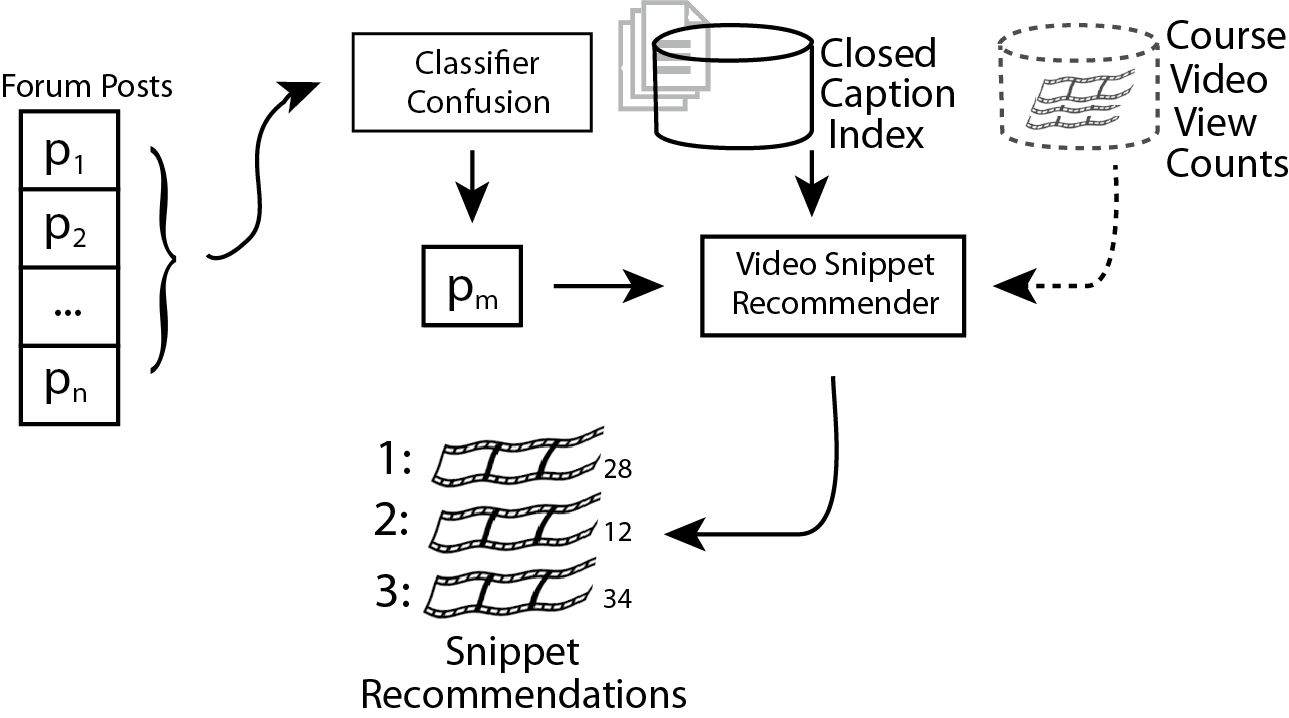
\includegraphics[width=0.5\textwidth]{../Figs/youEduArch.png}
       \caption{\textnormal{YouEDU Architecture. The YouEDU pipeline consists of two phases: post classification and video snippet recommendation.}}
       \label{figure:architecture}
\end{figure}

The second phase takes $P_{c}$ as input and, for each confused post in $p \in P_{c}$, outputs a ranked list of educational video snippets that address the object of confusion expressed in $p$. In particular, for a given post, the recommender produces an initial ranking across a number of one-minute video clips by computing a similarity metric between the post and closed caption sections. The ranking of videos in the retrieved set is then further informed by video-clickstream data.

While YouEDU outputs minute-resolution video clips, it does not necessarily guarantee that these clips fully address the exhibited confusion -- indeed, several minutes of instructional content are often required to explain a single concept. Rather, the video snippets collectively form an ad-hoc index. For example, say that for a given post, YouEDU outputs three video snippets with start times $s_{1}, s_{2}, s_{3}$, in order of decreasing relevance, and say that these snippets were contained in videos $v_{1}, v_{2}, v_{3}$, respectively, $v_{1}, v_{2}, v_{3}$ not necessarily unique. In order to clarify his or her confusion, the author of the post should begin watching video $v_{1}$ at $s_{1}$ -- the learner can autonomously set the end time of the snippet, and can move on to the next video, start time pair if any confusion still lingers. 

In the following two sections, we delve further into both phases of YouEDU, describing them in detail and relating the results of empirical evaluations.

\section{Phase I: Detecting Confusion}
\label{sec:confusionDetection}

% TODO: Cite
We frame the problem of detecting confusion as a binary one: Given a discussion forum post $p$ with a true label $L$ in \{not confused, confused\}, apply some hypothesis $h$ that correctly divines $L$. Posts with a confusion rating greater than four in the MOOCPosts dataset fall into the ``confused'' class, while all other posts fall into the ``not confused'' class.

We craft a rich feature space that fully utilizes the data available in our MOOCPosts dataset, choosing logistic regression with $l_{2}$ regularization as our statistical model. Results from empirical evaluations demonstrate that our classifier performs reasonably well, while simultaneously providing insight into the nature of confusion across multiple courses.

\subsection{Feature Space and Model Design}
Our feature space is composed of three types of inputs, those derived from: the post body; post metadata; and other classifiers. The confusion classifer we train functions as a combining layer that folds in the predictions of other classifiers; these classifiers are trained to predict variables correlated with confusion. We expand upon each type of input here.

\subsubsection{Bag-of-Words}
We take the bag-of-words approach in representing documents, or forum posts. Each document is represented in part as a vector of indicator variables, one for each word that appears in the training data -- the $i$-th indicator is one if the $i$-th word in the vocabulary is present in the document, zero otherwise. A word is defined as either a sequence of one or more alphanumeric characters or a single punctuation character (one of \{. , ; ! ?\}).

Documents are pre-processed before they are mapped to vectors. We prune out stop words, using a subset of the stop word list published by the Information Retrieval Group at the University of Glasgow \cite{glasgow}. Removed words inlcude, but are not limited to, interrogatives (``who'', ``what'', ``where'', ``when'', ``why'', ``how''), words that identify the self (``I'', ``my''), verbs indicating ability or the lack thereof, negative words (``cant'', ``cannot'', ``couldnt''), and certain conjunctions (``yet'', ``but''). We ignore alphabetic case\footnote{All-caps discussion certainly does communicate affect in some Internet forums -- it is typically associated with aggression and is considered a breach of ``nettiquette'' \cite{hambridge1995netiquette}; however, we assume that MOOC forum-goers are somewhat civil, and so accounting for case would needlessly inflate our feature space.} and lemmatize numbers, \LaTeX\ equations, and URLs. Intuitively, the presence of numbers and equations in a forum post might indirectly convey confusion or the lack thereof, in that the learner may be asking a question about some quantity or perhaps providing an answer to a quantitative question; similarly, a knowledgeable learner might answer a question by citing a URL. 

The unigram document representation, while simple, pervades text classification and often achieves high performance \cite{boulis2005text}. We employ $l_{2}$ regularization in order to prevent overfitting, a risk that is aggravated when the dimension of the feature space exceeds the training set size \cite{Ng:2004:FSL:1015330.1015435}.

\subsubsection{Post Metadata}
The feature vector derived from unigrams is augmented with post metadata, including: 
\vspace{-15pt}
\begin{itemize}
\setlength\itemsep{0.05em}
       \item The number of up-votes accumulated by the post. We rationalized that learners might express interest in posts that voiced confusion that they shared. 
       \item The number of reads garnered by the post's containing thread.
       \item Whether the poster elected to appear anonymous to his or her peers or to the entire population. It has been shown that anonymity in educational discussion forums enables learners to ask questions without fear of judgement \cite{freeman2004student}, and our dataset demonstrates a strong correlation between questions and confusion.
       \item The post author's grade in the class at the time of post submission, where ``grade'' is defined as the numer of points earned by the learner (e.g., by correctly answering quiz questions) divided by the number of points possible. The lower the grade, we hypothesized, the more likely the learner might be confused about a topic.
       \item The post position -- that is, whether or not the post was the first message in a thread. In order to seek help on a forum, a learner must first a post; most likely, we hypothesized, the learner will create a new thread for that post.
\end{itemize}

\subsubsection{Classifier Combination}
In section 3.2, we demonstrated that, at least in the humanities and medicine courses, confusion is significantly correlated with questions, answers, urgency, sentiment and opinion. As such, in predicting confusion, we take into account the predictions of five distinct classifiers, one for each of the aforementioned variables. We use the fine-grained method of combining classifiers in which the outputs of several classifiers are fed as input to a \emph{combination function} \cite{bennett2005combination}. In our case, the combination function is itself a classifier.

For a given train-test partition, let $D_{train}$ be the training set and $D_{test}$ be the test set. In both sets, each example is tagged along the six variables. Let $H_{q}$, $H_{a}$, $H_{o}$, $H_{s}$, and $H_{u}$ be classifiers for the question, answer, opinion, sentiment, and urgency variables, respectively. We call these classifiers \emph{constituent} classifiers. Each constituent is trained on $D_{train}$, taking as input bag-of-words and post metadata features, as described in the previous two subsections. 

Let $H_{c}$, a classifier for confusion, be our combination function. Like the constituent classifiers, $H_{c}$ is trained on $D_{train}$ and takes as input bag-of-words and metadata features. Unlike the constituents, $H_{c}$ also treats the ground-truth labels for the question, answer, opinion, sentiment, and urgency variables as features. When testing $H_{c}$ on an example $d \in D_{test}$, the constituent classifiers each output a prediction for $d$. These five predictions are appended to the bag-of-words and metadata features derived from $d$. The resulting vector is given as input to $H_{c}$, which then predicts $d$'s confusion class.

A few subtleties: $H_{s}$ uses an additional metadata feature that the other classifiers do not -- the number of negative words (e.g., ``not'', ``cannot'', ``never'', etc.). $H_{q}$, $H_{a}$, $H_{u}$, and $H_{c}$ treat the number of question marks as an additional feature, given the previously presented correlations; \cite{wen2015confusion} also used question marks in predicting confusion. And while $H_{q}$, $H_{a}$, and $H_{o}$ are by nature binary classifiers, $H_{s}$ and $H_{u}$ are multi-class. They predict values corresponding to negative (raw score $< 4$), neutral (raw score $= 4$), and positive (raw score $> 4$), in order to provide $H_{c}$ with somewhat granular information.

\subsection{Evaluation and Discussion}
For clarity, we refer to the confusion classifier that uses all the features
described in the section 5.1 as the \emph{combined} classifier. In this section, we evaluate and interpret the performance of both the combined classifier and confusion classifiers with pared-down feature sets, reporting insights and intuitions gleaned about the nature of confusion in MOOCs along the way. 

\begin{table*}[htp!]
    \centering
    \begin{tabular}{|c|c c c|c c c|c|}
    \hline
    \multirow{2}{*}{Course Set} & \multicolumn{3}{c|}{Not Confused} & \multicolumn{3}{c|}{Confused}  & \multirow{2}{*}{Kappa} \\ \cline{2-7}
                                &  Precision & Recall & $F_{1}$     &  Precision & Recall & $F_{1}$  &       \\ \hline
    Humanities                  & 0.898      & 0.943    & 0.919     & 0.778      & 0.642  & 0.700    & 0.621  \\ \hline
    Medicine                    & 0.924      & 0.946    & 0.935     & 0.699      & 0.589  & 0.627    & 0.564  \\ \hline

    \end{tabular}
    \caption{\textnormal{
       Combined Confusion Classifier Performance, Course Sets. For each course set listed, this table reports the average performance across 10 folds of stratified cross-validation.
    }} % title of Table
    \label{table:confusion_sets} % is used to refer this table in the text
\end{table*}

We quantify performance primarily using two metrics: $F_{1}$ and Cohen's Kappa. We favor the Kappa over accuracy because the former accounts for chance agreement \cite{cohen1960coefficient}. Unless stated otherwise, reported metrics represent an average over 10 folds of stratified cross-validation. 

\subsubsection{Confusion at the Course-Set Granularity}
Table \ref{table:confusion_sets} presents the performance of the combined classifier on the humanities and medicine course sets. As mentioned in section 3.1, both sets are somewhat heterogenous collections of courses, with a total nearly 10,000 posts in each set. In our dataset, not-confused posts outnumber confused ones -- in the humanities course set, but 23\% of posts exhibit confusion, and in the medicine course set, 16\% do. As such, our classifier was naturally better at identifying non-confused posts than confused posts.

\subsubsection{The Language of Confusion Across Courses}

\begin{table*}
       \centering
       \begin{tabular}{|c|c|c|c|c|}
       \hline
       Course                         & \# Posts (\% Confused) & $F_{1}$: Not Confused & $F_{1}$: Confused & Kappa \\ \hline
       Managing Emergencies              & 279 (18\%)                         & 0.963                 & 0.771             & 0.741 \\ \hline
       Statistical Learning              & 3,030 (30\%)                        & 0.909                 & 0.767             & 0.677 \\ \hline
       Economics 1                       & 1,583 (23\%)                     & 0.933                 & 0.741             & 0.675 \\ \hline
       Statistics in Medicine (2014)     & 1,218 (28\%)                        & 0.908                 & 0.748             & 0.658 \\ \hline
       Statistics in Medicine (2013)     & 3,320 (21\%)                         & 0.916                 & 0.671             & 0.589 \\ \hline
       Science Writing                   & 5,181 (10\%)                         & 0.961                 & 0.527             & 0.491 \\ \hline
       Women's Health                    & 2,141 (15\%)                         & 0.933                 & 0.506             & 0.445 \\ \hline
       How to Learn Math                 & 9,878 (6\%)                        & 0.970                 & 0.383             & 0.359 \\ \hline
       \end{tabular}
       \caption{\textnormal{
       Combined Confusion Classifier Performance, Individual Courses. Our classifier performed best on courses whose discourse was characterized by technical diction, like statistics or economics. In courses like \emph{How to Learn Math} that facilitated open-ended and somewhat roaming discussions, our model found it more difficult to implicitly define confusion. 
       }} % title of Table
       \label{table:confusion_courses} % is used to refer this table in the text
\end{table*}

Table \ref{table:confusion_courses} presents the performance of the combined classifier on select courses, sorted in descending order by Kappa. Our classifier performed best on courses that traded in highly technical language. Take, for example, the following two posts from \emph{Managing Emergencies}:

\vspace{-10pt}
\begin{displayquote}
What could have caused the hemoptysis in this patient with pnuemonia?
\end{displayquote}
\vspace{-10pt}

\vspace{-5pt}
\begin{displayquote}
At what doses is it therapuetic for such a patient because at high doses it causes vasoconstrition through alpha1 interactions, while at low doses it causes dilation of renal veins and splachinic vessels.
\end{displayquote}
\vspace{-10pt}

Both of these posts were tagged as exhibiting confusion, and both of them are fairly saturated with medical terms. Incidentally, our classifier achieved its highest performance when cross-validating on this course (Kappa = 0.741). This makes intuitive sense -- a vocabulary so technical and esoteric is likely only used when a learner is discussing or asking a question about a specific course topic. Indeed, inspecting our model's weights revealed that ``systematic'' was the $11^{th}$ most indicative feature for confusion (odds ratio = 1.23) and ``defibrillation'' was the $15^{th}$ (odds ratio = 1.22). Similarly, in \emph{Statistical Learning}, ``solutions'' was the sixth most indicative feature for confusion (odds ratio = 1.75), and``predict'' was the ninth (odds ratio = 1.65).

A glance at Table \ref{table:confusion_courses} suggests that our classifier's performance degrades as the discourse becomes less technical. Posts like the following were typical in \emph{How to Learn Math}, an education course about the pedagogy of mathematics:

\vspace{-10pt}
\begin{displayquote}
I am not sure if I agree with tracking or not.  I like teaching children at all levels.  It seems that if you teach kids at the same level then it becomes the Sam ethnic \emph{[sic]} over and over.  ...  In a normal class setting the lower level learners can learn from the higher learners and vice versa.  Although I do find it very hard to find a middle ground. There has to be an easier way.
\vspace{-10pt}
\end{displayquote}

The above post was tagged as exhibiting confusion, but the language is much more subtle than that seen in the posts from \emph{Managing Emergencies}. In technical courses, there was a sharp shift in diction between confused posts and not-confused posts. The same could not necessarily be said for non-technical courses, and it is not surprising that we saw our lowest Kappa (0.359) when classifying \emph{How to Learn Math}. Indeed, in the education course, learners tend to voice more confusion about the structure of the class than the content itself -- ``link'', ``videos'', and ``responses'' are the fourth, fifth, and seventh most indicative features for the confusion class, respectively.

Examining the feature weights learned when cross-validating on the humanities and medicine course sets provides us with a more holistic view onto the language of confusion. Domain-specific words take the backseat to words that convey the learning process. For example, in both course sets, ``confused'' was the word with the highest feature weight (odds ratios equal to 3.19 and 2.97 for humanities and medicine, respectively). In the humanities course set, ``?'', ``couldn't'', ``question'', ``haven't'', and ``wondering'' came next, in that order. The importance of question-related features in particular is consistent with \cite{wilson1989learning} and with the correlations in the MOOCPosts dataset. In medicine, the next highest ranked words were ``explain'', ``role'', ``understand'', ``stuck'', and ``struggling''.

Table \ref{table:informative_features} displays the most informative features for humanities and medicine course sets, as well as \emph{How to Learn Math} and \emph{Managing Emergencies}.
\begin{table*}[ht!]
       \centering
       \begin{tabular}{|c|c|c|c|}
       \hline
       Humanities                  & Medicine              & How to Learn Math         & Managing Emergencies \\ \hline
       constituent:urgency (6.59)         & constituent:question (4.05) &  constituent:question (6.64)    & constituent:urgency (2.47)  \\ \hline
       constituent:question (3.47)       & confused             (2.98) &  constituent:urgency   (2.13)   & constituent:question (2.34) \\ \hline
       confused             (3.20)      & explain               (2.71) &  hoping                (1.94)   & ? (1.73) \\ \hline
       ?                    (3.14)       & role                 (2.41) &  link                  (1.76)  & metadata:\#? (1.54) \\ \hline
       couldn't             (2.40)      & understand            (2.36) &  available             (1.63)   & hope (1.40) \\ \hline
       report               (2.23)       & stuck                (2.27) &  responses             (1.62)   & what (1.31) \\ \hline
       manual               (1.94)       & struggling           (2.25) &  middle                (1.62)   & understand (1.29) \\ \hline
       question             (1.91)       & constituent:urgency  (2.25) &  support               (1.60)  & dr (1.24) \\ \hline
       haven't              (1.84)       & sentence             (2.20) &  discussing            (1.60)   & how (1.24) \\ \hline
       wondering            (1.83)       & little               (2.09) &  instruction           (1.60)  & meant (1.23) \\ \hline
       \end{tabular}
       \caption{\textnormal{
       Most Informative Features, Odds Ratios. Features prefixed with ``constituent:'' correspond to constituent predictions, while those prefixed with ``metadata'' correspond to post metadata features. All other features are unigram words.
       }} % title of Table
       \label{table:informative_features} % is used to refer this table in the text
\end{table*}

\subsubsection{Training and Testing on Distinct Courses}
We ran a series of experiments in which we trained the combined classifier on posts from one course and then tested it on posts from another one, without cross-validation. The results of these experiments are tabulated in Table \ref{table:across_courses}. 

\begin{table}[]
       \centering
       \begin{tabular}{|c|c|c|}
       \hline
       Training Course                & Test Course                    & Kappa \\ \hline
       Stats. in Medicine (2013)  & Stats. in Medicine (2014)  & 0.629 \\ \hline
       Stat. Learning           & Stats. 216                 & 0.590 \\ \hline
       Economics 1                    & Stats. in Medicine (2013)  & 0.267 \\ \hline
       Stats. in Medicine (2013)  & Women's Health                 & 0.175 \\ \hline
       \end{tabular}
       \caption{\textnormal{
       Nature of Confusion Across Domains. Training and testing on similar courses typically resulted in high performance, especially in the case of technical courses.
       }} 
       \label{table:across_courses} % is used to refer this table in the text
\end{table}


Our highest Kappa (0.629) was achieved when training on \emph{Statistics in Medicine 2013} and testing on \emph{Statistics in Medicine 2014}; this makes sense, since they comprise two runs of the same course. Many instructors plan to offer the same MOOC multiple times \cite{hollands2014moocs}. If an instructor could tag but one of those runs, then a classifier like ours deployed in an online setting might be met with success. Even if that tagging process is too expensive, our results when training on \emph{Statistical Learning} and testing on \emph{Statistics 216} suggest that an online classifier might perform well so long as its training data derives from the same domain as the test data. Performance might suffer, however, if the domains of the training and test data are non-overlapping, as is the case in the last two experiments in Table \ref{table:across_courses}.

\subsubsection{Constituent Classifiers and Post Metadata}

\begin{figure}
\vspace{-18pt}
       \centering
       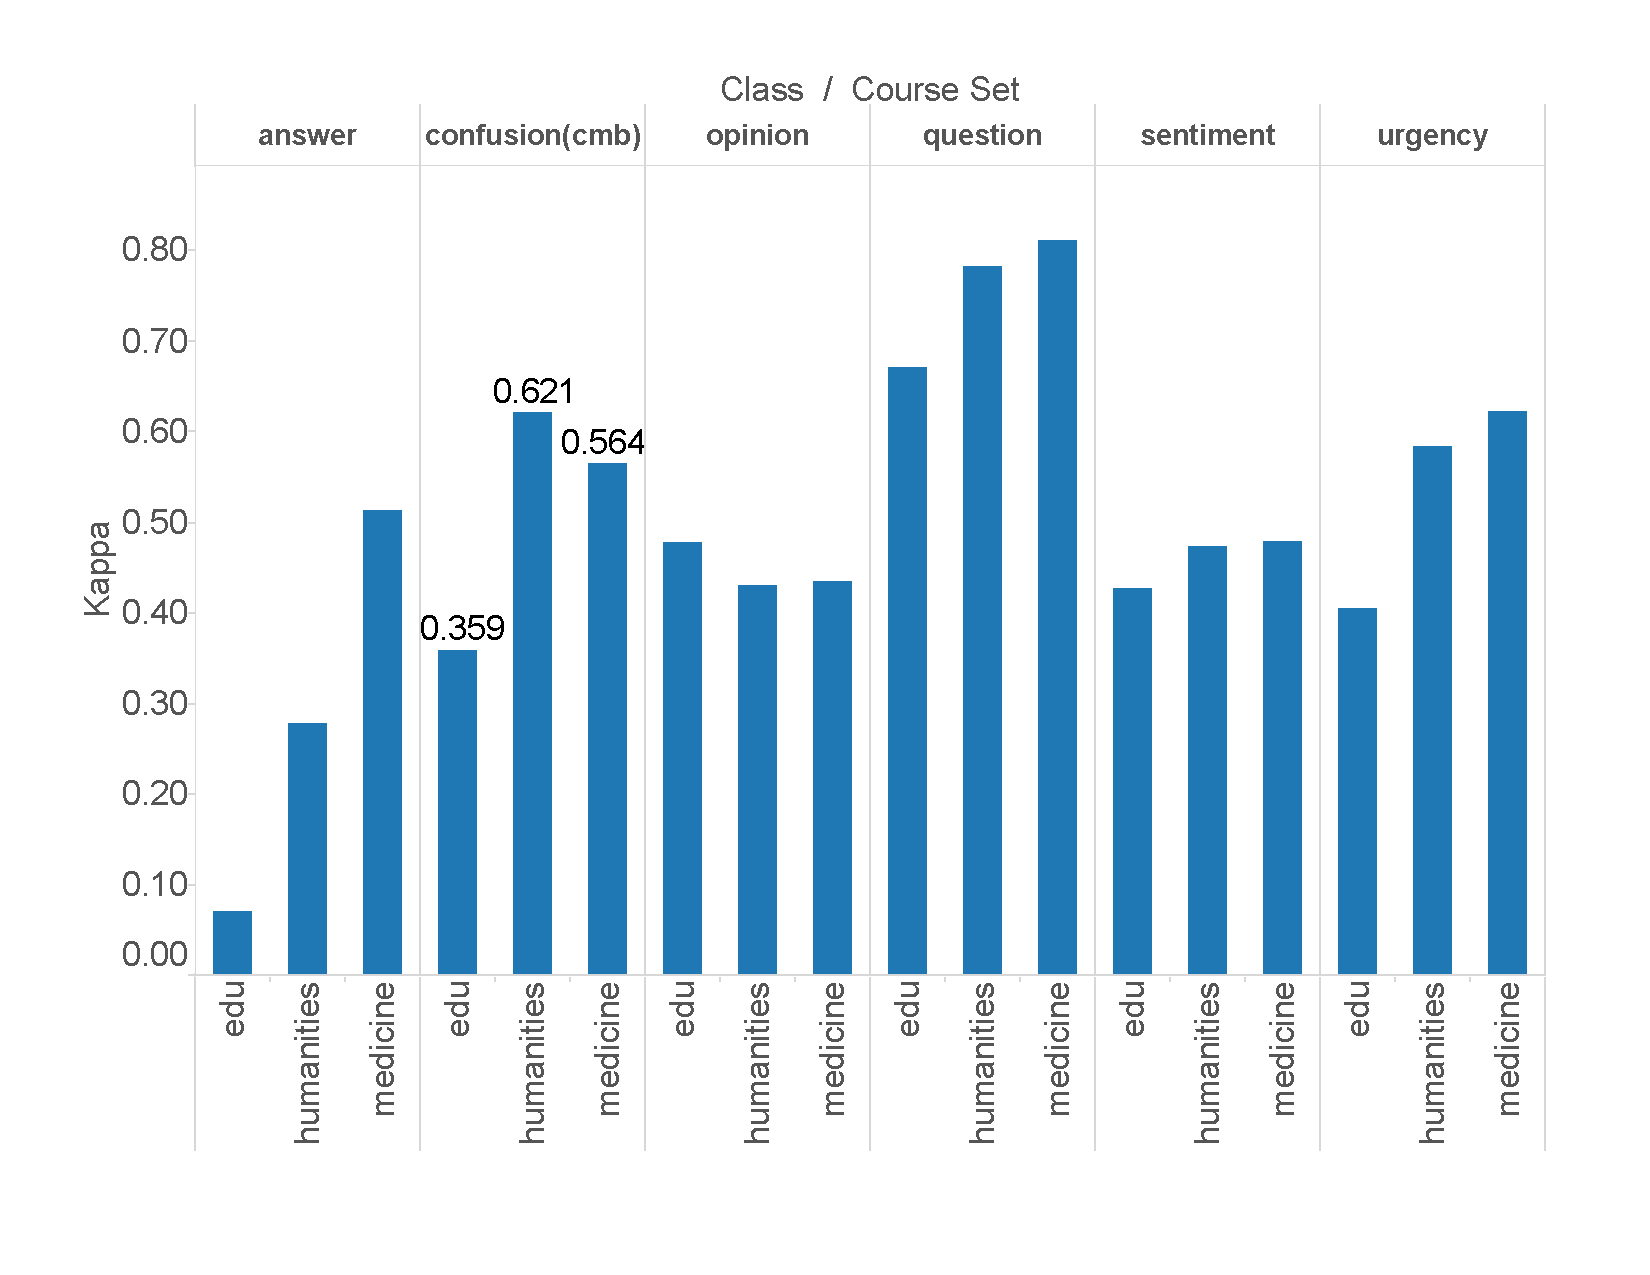
\includegraphics[width=0.5\textwidth]{../Figs/classifierEvalsWithEduAltLayout.pdf}
       \vspace{-30pt}
       \caption{\textnormal{Constituent Classifier Performance. This figure visualizes the performance of the constituent classifiers, as well as the performance of the combined classifier (confusion(cmb), where ``cmb'' is short for combined).}}
      \label{figure:constituents}
\end{figure}

Figure \ref{figure:constituents} illustrates the performance of each constituent classifier when cross-validating on the humanities and medicine course sets, as well as on the education course. The constituent question classifier outperforms all the others by a large margin, likely because the structure of questions is fairly consistent. (Note that the constituent classifiers are not themselves fed by a lower level of classifiers; if we were attempting to predict, say, sentiment instead of confusion, we could try to improve over the performance shown here by creating a sentiment combination function that was informed by its own set of constituent classifiers.)

\begin{table}
       \centering
       \begin{tabular}{|c|c|c|c|}
       \hline
       Course Set           & Humanities & Medicine & Learn Math \\ \hline
       Combined Classifier  & 0.621      & 0.564    & 0.359 \\ \hline\hline
       Minus Question       & 0.621      & 0.559    & 0.350 \\ \hline
       Minus Answer         & 0.620      & 0.555    & 0.345 \\ \hline
       Minus Opinion        & 0.619      & 0.553    & 0.310 \\ \hline
       Minus Sentiment      & 0.621      & 0.555    & 0.292 \\ \hline
       Minus Urgency        & 0.618      & 0.512    & 0.337 \\ \hline
       Minus Post Position      & 0.614      & 0.482    & 0.337 \\ \hline
       \end{tabular}
       \caption{\textnormal{
       Ablative Analysis, Kappas. Minus question is the combined classifier without the constituent question classifier; minus answer is the minus question classifier without the constituent answer classifier; and so on.
       }} % title of Table
       \label{table:ablative} % is used to refer this table in the text
\end{table}

The combining fuction of our combined classifier consistently determined that the constituent classifiers for the question and urgency variables were particularly indicative of confusion (see Table \ref{table:informative_features}). Table \ref{table:ablative} shows the results of an ablative analysis in which one constituent classifier was removed from the combined classifier at a time, until we were left with a classifier with no constituent classifiers (call it a \emph{flat} classifier). The flat classifier performed worse than the combined classifier in the two course sets and the education course, with the drop in performance most pronounced in the medicine course set. For both course sets, the urgency constituent seemed to be the most helpful of the five constituents -- this makes intuitive sense, since we would expect that instructors would prioritize posts in which learners were struggling to understand the course material. However, the same was not true for \emph{How to Learn Math}, which is consistent with the fact that no significant correlation between confusion and urgency was found (see section 3.2).

The post position metadata feature also contributed positively to the classifier's performance -- removing it from the flat classifier for medicine dropped the Kappa by 0.03. The other metadata features, however, did not appear to consistently or appreciably affect classifier performance, and so we chose to omit them from our ablative analysis.

Table \ref{table:informative_features} shows that the number of question marks was also an informative feature, at least in the \emph{Managing Emergencies} course. 

\section{Phase II: Recommending Clips}
\label{sec:clipRecommendation}
\subsection{The Recommendation Algorithm}
\subsubsection{Retrieval}
\subsubsection{Ranking}

\subsection{Evaluation}
Two experts were hired ...

\section{Future Work}
\label{sec:futureWork}

Future work might focus on strengthening the link between the classifiers and the reccomendation system; in particular, it would behoove us to devise a way to filter our set of confused posts to a subset for which recommendation makes sense. Additionally, we might want to make our classifiers better and index back into the previous course to retrieve answers for courses. Deploying this system live is another thing that we might do. 

YouEDU's two phases need not be packaged together; in an online setting, they could operate as independent, complemetary services. The output of Phase I could be presented directly to instructors, many of whom express interest in understanding activity in discussion forums \cite{Stephens-Martinez:2014:MMI:2556325.2566246}. As for Phase II, the recommendation system might live as a search-box of sorts: learner would type natural language queries in which they voiced their confusion, and our system would serve them relevant resources.

\section{Conclusion}
\label{sec:conclusion}

YouEDU takes an initial step towards building automated confusion intervention ... 

%\end{document}  % This is where a 'short' article might terminate

%ACKNOWLEDGMENTS are optional
\section{Acknowledgments}
This section is optional\cite{wen2014sentiment}; it is a location for you
to acknowledge grants, funding, editing assistance and
what have you.  In the present case, for example, the
authors would like to thank Gerald Murray of ACM for
his help in codifying this \textit{Author's Guide}
and the \textbf{.cls} and \textbf{.tex} files that it describes.

%
% The following two commands are all you need in the
% initial runs of your .tex file to
% produce the bibliography for the citations in your paper.
\bibliographystyle{abbrv}
\bibliography{sources}  % sigproc.bib is the name of the Bibliography in this case
% You must have a proper ".bib" file
%  and remember to run:
% latex bibtex latex latex
% to resolve all references
%
% ACM needs 'a single self-contained file'!
%
%APPENDICES are optional
%\balancecolumns
\balancecolumns
% That's all folks!
\end{document}
